\documentclass{article}
\usepackage{graphicx}
\usepackage{hyperref}
\title{Konkurrensanalys}
\author{Vanessa \textsc{Rojas}}
\date{\today}


\begin{document}

\maketitle

\section{Appar}

2 konkurrerande appar 

\subsection{App: Itemtopia}

\url{https://itemtopia.com/}

Itemtopia är en app där användare kan spara sina ägodelar och lägga till information om dem (anteckningar, kvitton, bilder). Appen fokuserar mest på ägodelars beskrivningar och detaljer.

\subsection{App: Magic Home Inventory}

\url{http://www.twisterrob.net/project/inventory/}

Magic Home Inventory är en app där användare kan göra en inventarie av sina ägodelar. Appen fokuserar mest på placering och struktur.

\section{Krav}

\subsection{Måste-krav (båda appar):}
\begin{enumerate}
\item En användare ska kunna lägga till olika ägodel-element med namn och anteckningar för att representera riktiga ägodelar.
\item En användare ska kunna se en lista med de sparade ägodel-elementen för att se vad som lades till.
En användare ska kunna lätt identifiera element i listan för att få en översikt.
\item En användare ska kunna klicka på ett element i listan för att se mer information om elementet.
\item En användare ska kunna söka ägodelar med namn för att hitta dem och se information om dem.
\item En användare ska kunna redigera element för att ändra information om dem.
\item En användare ska kunna ta bort element som inte längre önskas.
\end{enumerate}

\subsection{Egna-krav (Itemtopia):}
\begin{enumerate}
\item En användare ska kunna lägga till behållare-element (egendom, extra mapp) som får innehålla andra element i sig.
\item En användare ska kunna skapa ett konto och logga in för att spara och ha tillgång till sina ägodelar.
\item En användare ska kunna lägga till bilder, kvitton, handböcker, extra anteckningar och dokument för att komplettera information om ett element.
\item En användare ska kunna välja mallar till element när ett element skapas för att förenkla skapande och sökande. Till exempel kan en användare välja "elektroniska komponenter" och få en ikon och fält som passar en elektronisk komponent.
\end{enumerate}

\subsection{Egna-krav (Magic Home Inventory):}
\begin{enumerate}
\item En användare ska kunna lägga till olika djup på behållare-element (hus, rum, hyllor, lådor) som får innehålla andra element i sig.
\item En användare ska kunna lägga till bilder och anteckningar för att komplettera information om ett element.
\item En användare ska kunna flytta ett element till ett annat behållare-element.
\item En användare ska kunna säkerhetskopiera sina element.
\item En användare ska kunna placera element i flera kategorier för att förenkla sökande.
\end{enumerate}


\section{UI}

\subsection{Itemtopia}

\begin{figure}
\begin{center}
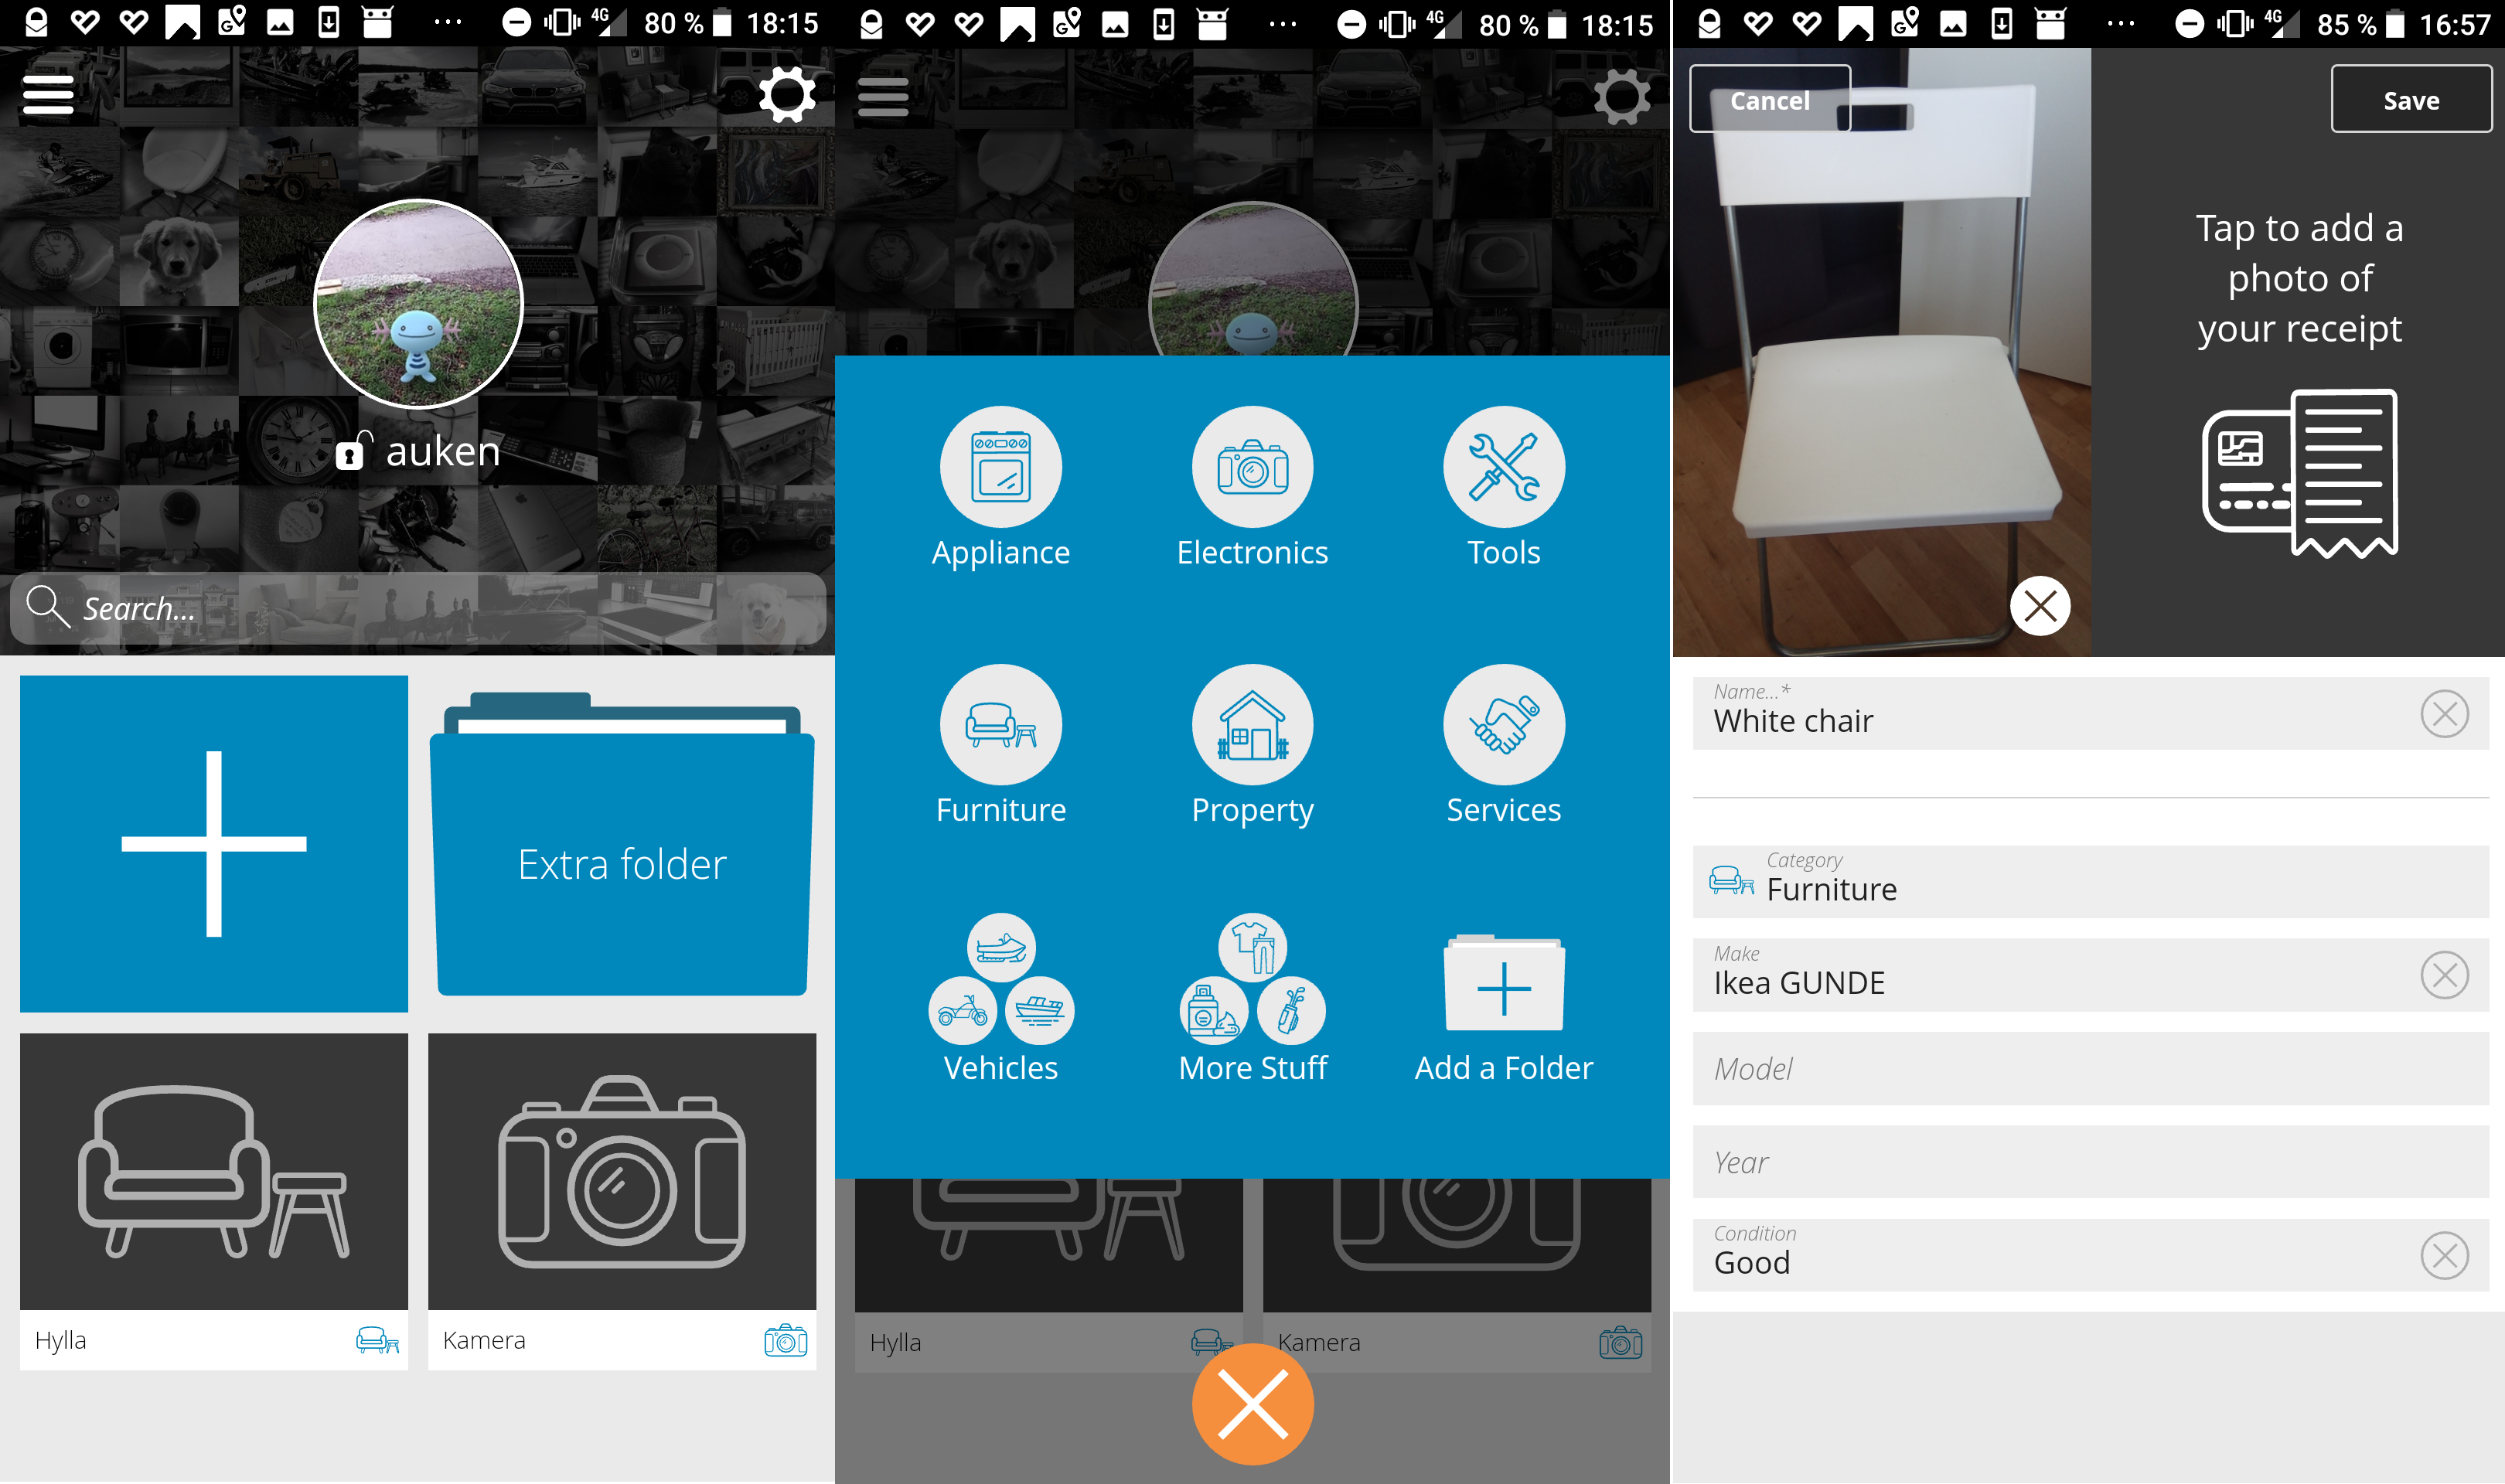
\includegraphics[width=1\textwidth]{itemtopia} 
\caption{Itemtopia: a) Lista med element och mapp. b) Lägga till element med en mall. c) Lägga till bilder och extra information till element.}
\end{center}
\end{figure}

\subsection{Magic Home Inventory}

\begin{figure}
\begin{center}
\includegraphics[width=1\textwidth]{inventory} 
\caption{Magic Home Inventory: a) Lista med element och mapp. b) Flytta element till en annan plats. c) Söka element.}
\end{center}
\end{figure}

\end{document}
